
\chapter{Superhydrophobic Droplet Impact - Comparison with Gerris simulations}

\section{Contact angle}
\begin{wrapfigure}{r}{0.5\textwidth}
  \begin{center}
    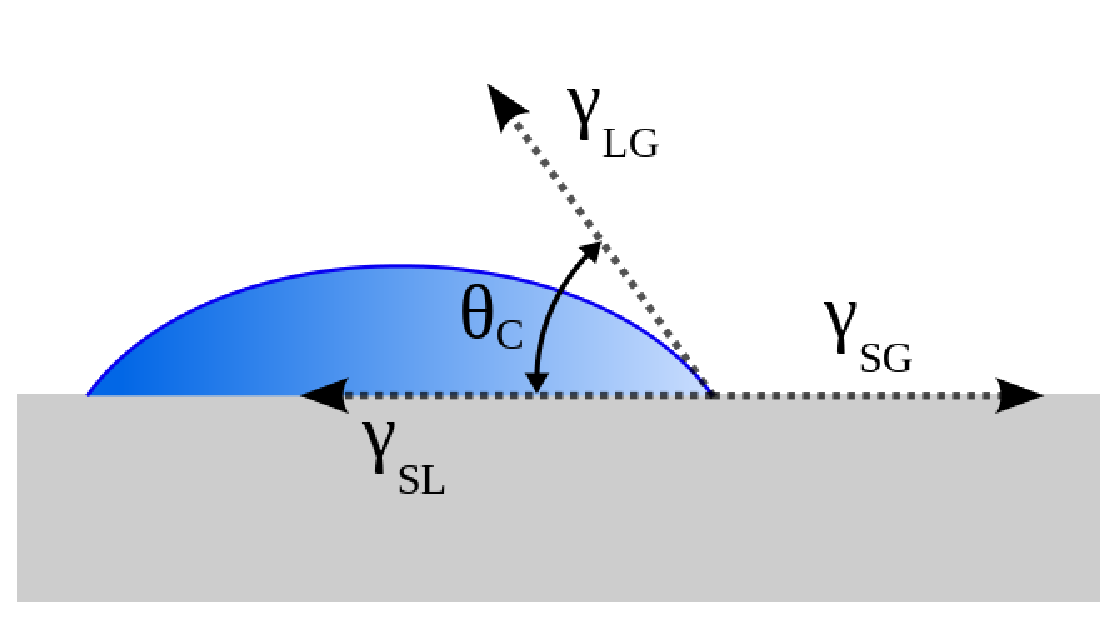
\includegraphics[width=0.48\textwidth]{Contact_angle.eps}
  \end{center}
  \caption{Contact Angle}
  \label{Fig:Contact_angle}
\end{wrapfigure}
When a gas-liquid interface meets a solid surface, at the point of contact of three phases the liquid makes an angle with the surface. This measures the wettability of 
the solid surface for that liquid. The contact angle is given by Youngs equation, ( See Figure \ref{Fig:Contact_angle} ). 
\begin{equation}
 \boxed{ \begin{align}
 &\gamma_{SG} -\gamma_{SL} - \gamma_{LG} \cos \theta =0  \\
 &\cos \theta =\frac{\gamma_{SG} -\gamma_{SL}}{\gamma_{LG}} 
 \end{align}
 }
 \label{Eq:youngs}
\end{equation}
which expresses the balance of forces acting on the contact line in the direction normal to the contact line and tangential
to the solid surface. Experiments show that the contact angle deviates from its static value when
the contact line is in motion.This deviation is an important feature of the problem and needs to be taken into account to obtain realistic answers. \\
\\
\underline{\textbf{Superhydrophobic surfaces}}\\
The effect of the dynamic contact angle and moving contact line however can be made minimal if the spreading of the droplet is very less. Such phenomenon is seen in non-wetting surfaces. 
Surfaces which are extremely difficult to wet are known as superhydrophobic surfaces. \cite{wang2007definition} has attempted to define the superhydrophobic surfaces as the
surfaces that exhibit static contact angle greater than $150^o$. In the next sections we compared some experimental studies on superhydrophobic surfaces with simulations done on Gerris.
% \begin{figure}
% \centering
%     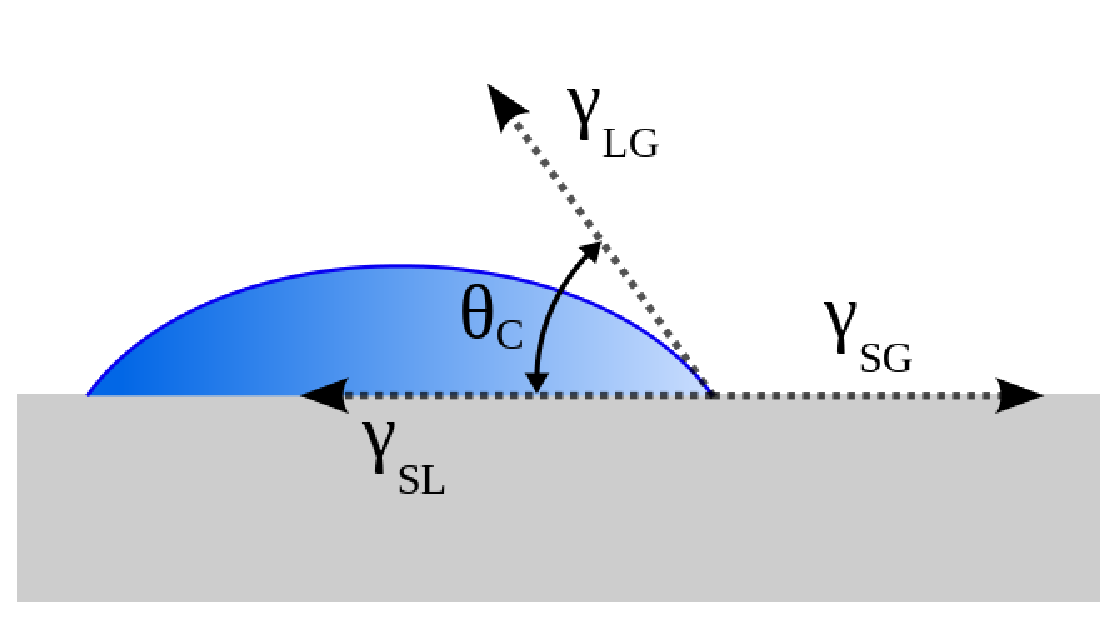
\includegraphics[width=0.48\textwidth]{Contact_angle.eps}
%   \caption{Contact angle}
%   \label{Fig:Contact_angle}
% \end{figure}

\section{Gerris}
Gerris is an open source code created by \cite{Popinet2003} which solves Navier stokes equation using a VOF method for constructing the interface.
However the units are non-dimensional, we can use any system of units, it have to be consistent throughout
the simulation file and the results will be in those units.

\begin{equation}
 \boxed{ \begin{align}
 \frac{d \overrightarrow u}{dt} &= \frac{1}{\rho} \left\{ - \overrightarrow \nabla p + \overrightarrow \nabla \cdot ( \mu (\overrightarrow \nabla \overrightarrow u + \nabla \overrightarrow u^T )) + \sigma \kappa \delta_s \overrightarrow n \right\} + { {\tt Source} }(\overrightarrow u)\\
 \overrightarrow \nabla . \overrightarrow u &= 0 \qquad\text{(Equation of continuity)}\\
\frac{DF}{Dt}&=0 \qquad\text{(Volume of Fluid advection equation)}
\end{align} }
\label{Eq:gerris}
\end{equation}

There are some limitations in Gerris flow solver
\begin{enumerate}
 \item No contact line model
 \item No dynamic contact angle model
\end{enumerate}

To know the effects of these two limitations, we compared the Gerris simulation with \cite{Hung2011}, \cite{Clanet2004} and \cite{Wang2007}
having no-slip conditions and static contact angle at the surface.
\section{Gerris Simulation}
To run simulations in we have to find the non dimensional parameters for our problem.
We use Buckingham $\pi$ method to find out number of non dimensional parameters ( See Table \ref{table:bp} )
\begin{table}
  \begin{center}
    \caption{Dimensional matrix to determine non-dimensional groups}
    \label{table:bp}
      \begin{tabular}{c c c c c c c c c c}
	\toprule
	Dimensional Variables & $\rho_L$ & $\rho_g$ & $\mu_L$ & $\mu_g$ & $\sigma_{Lg}$ & $L_b$ & $D_o$ & $H_o$ & $g$ \\
	\midrule
	M & 1 & 1 & 1 & 1 & 1 & 0 & 0 & 0 & 0 \\
	L & -3 & -3 & -1 & -1 & 0 & 1 & 1 & 1 & 1 \\
	T & 0 & 0 & -1 & -1& -2 & 0 & 0 & 0 & -2 \\
	\bottomrule
      \end{tabular}
     \end{center}
 \end{table}

Rank of the matrix = 3 \\

Number of independent non-dimensional parameters = 9-3 = 6 \\

Gerris simulation takes a dimensional input as parameters for density, viscosity of both fluids, surface tension and source term (generally gravitational acceleration. 
We can non-dimensionalise the equation \ref{Eq:gerris} which Gerris solves. We choose scales as characteristic length  L, characteristic velocity U,
characteristic time $\frac{L}{U}$, characteristic pressure $\rho_L U^2$, characteristic density $\rho_L$ and characteristic viscosity $\mu_L$.
Substitute $u = U\tilde u $, $x = L\tilde x $, $y = L\tilde y $, $t = \frac{L}{U}\tilde t $, $p = \rho_L U^2\tilde p $, $\rho = \rho_L \tilde\rho $, $\mu = \mu_L \tilde\mu $
in \ref{Eq:gerris}, where quantities with tilde are non-dimensional.

\begin{equation}
 \boxed {\begin{align}
 \frac{d \tilde u}{d\tilde t} &= \frac{1}{\rho_k} \left\{ - \tilde \nabla p + \frac{1}{Re_L}  \tilde \nabla \cdot ( \mu_k (\tilde \nabla \tilde u + \nabla \tilde u^T )) 
 + \frac{1}{We} \kappa \delta_s \overrightarrow n \right\} + \frac{1}{Fr^2} \\
 \tilde \nabla . \tilde u &= 0 \qquad\text{(Equation of continuity)}\\
 \frac{D\tilde F}{D\tilde t}&=0 \qquad\text{(Volume of Fluid advection equation)}
\end{align} }
\label{Eq:gerris_nd}
\end{equation}
where, $Re_L = \frac{L\rho_L U}{\mu_L}$ and $Fr = \frac{U}{\sqrt{gL}}$. \\

\underline{Domain} \\
The domain consists of three boxes and axis of symmetry lies on y-axis ( See Figure \ref{Fig:domain-gerris}), 
\begin{figure}[tbp]
\centering
 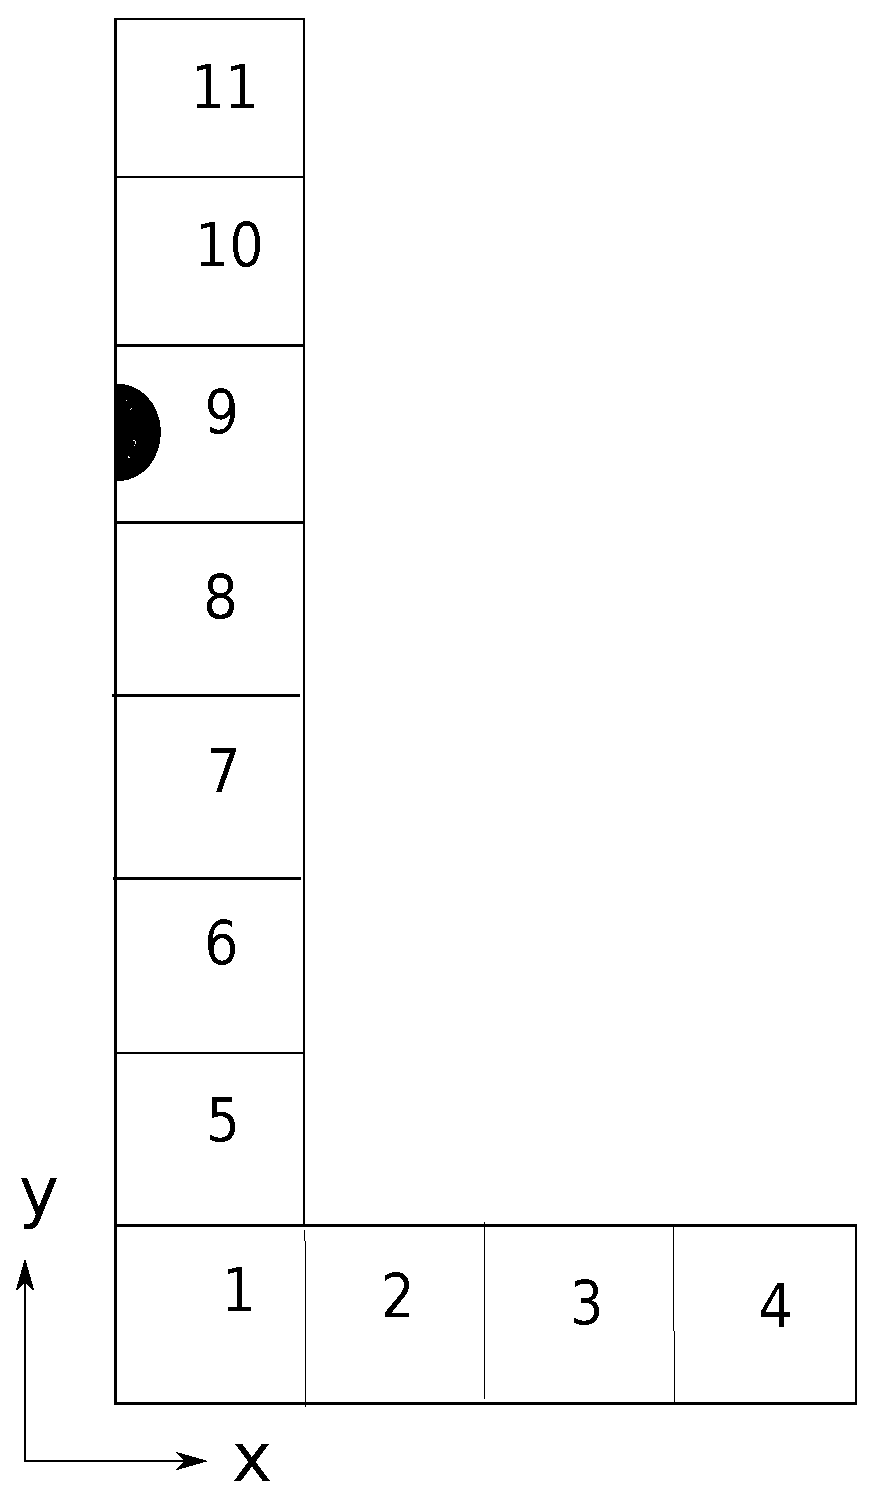
\includegraphics[scale = 0.5]{domain.eps}
 \caption{Domain for simulation (Axisymmetric)}
 \label{Fig:domain-gerris}
\end{figure}

 \begin{table}
  \begin{center}
   \caption{Input for non-dimensional simulation (Calculated from dimensional parameters as in \cite{Hung2011})}
 \label{Table:input}
    \begin{tabular}{lll}
      \toprule 
      Parameter & Remark & Value  \\ 
      \midrule
	Re & Reynolds number & 2521.285386 \\
	We & Weber number of Liquid-gas & 29.43 \\
	$H_k$ & $\frac{H_o}{D_o}$ &  12.00\\
	$L_k$ & $\frac{L_o}{D_o}$ &  2 \\
	$\rho_k$ & $\frac{\rho_g}{\rho_L}$ & $2 X 10^{-3}$  \\ 
	$\mu_k$ & $\frac{\mu_g}{\mu_L}$ & $2 X 10^{-2}$ \\
      
      \bottomrule \\
    \end{tabular}
  \end{center}
\end{table}

\underline{Initial Condition} \\
\begin{equation}
 x^2+(y+(H_k-0.5L_k))^2=0.25  %this equation is altered here from simulation there the axes are inverted
\end{equation}

\underline{Boundary Conditions}: No slip conditions on all walls except axis of symmetry where we use symmetry conditions(described in section \ref{sec:bc}). Impact surface
has a static contact angle of $150^o$.

\section{Results and Discussion}
\begin{figure}[H]
 \centering
 \subfloat[t = 0.0357 ]{%
      \includegraphics[width=0.3\textwidth]{hung-1.eps}
      }
  \subfloat[t = 0.0361 ]{%
      \includegraphics[width=0.3\textwidth]{hung-2.eps}
      } \\
       \subfloat[t = 0.0362 ]{%
      \includegraphics[width=0.3\textwidth]{hung-3.eps}
      }
       \subfloat[t = 0.0365 ]{%
      \includegraphics[width=0.3\textwidth]{hung-4.eps}
      }\\
    \subfloat[t = 0.0368 ]{%
      \includegraphics[width=0.3\textwidth]{hung-5.eps}
      }
       \subfloat[t = 0.0371 ]{%
      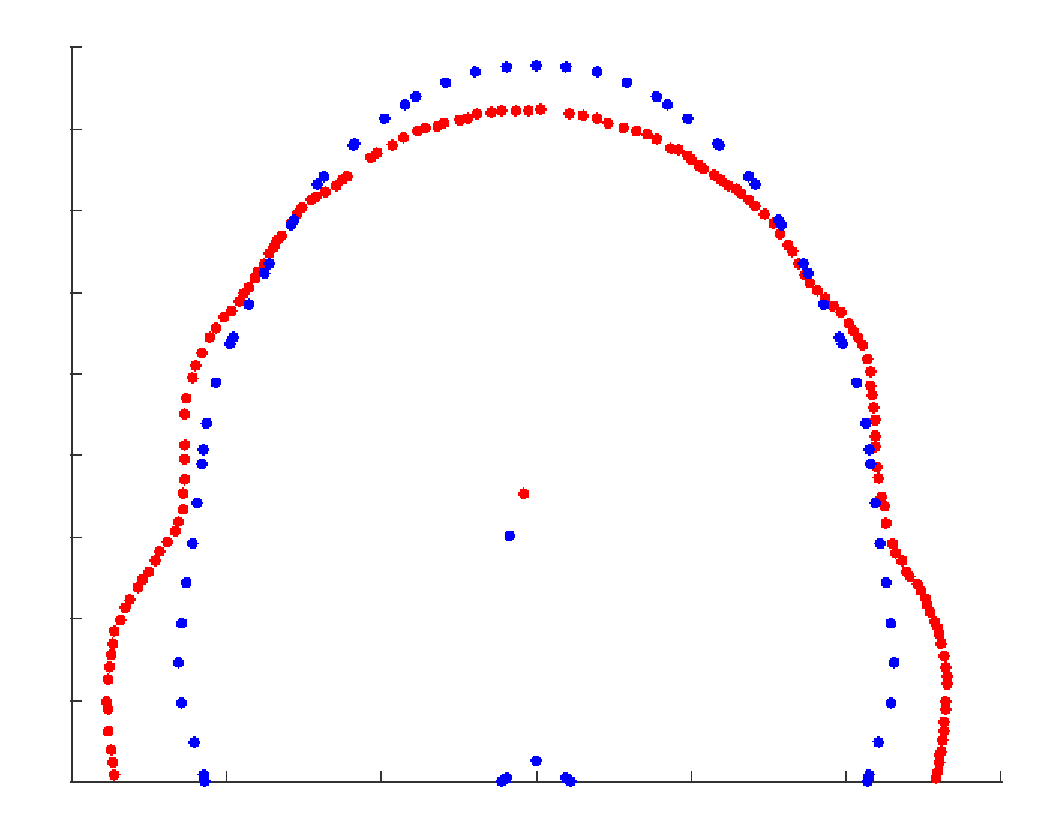
\includegraphics[width=0.3\textwidth]{hung-6.eps}
      }\\
       \subfloat[t = 0.0374 ]{%
      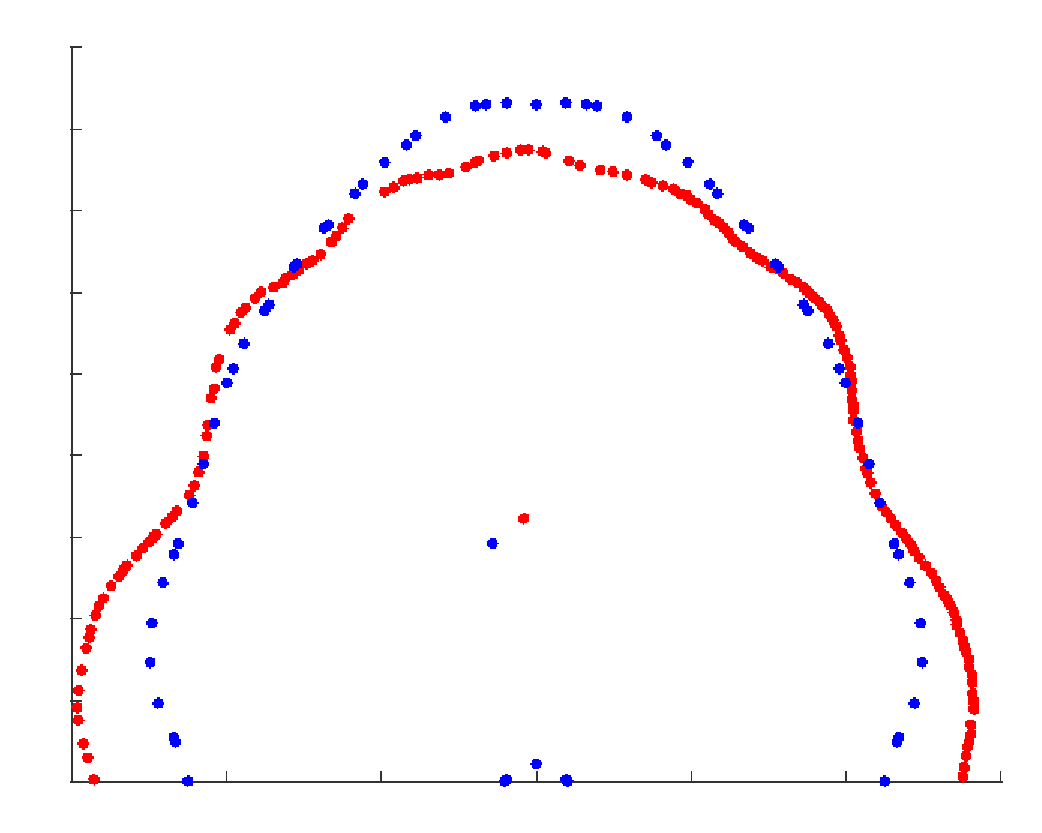
\includegraphics[width=0.3\textwidth]{hung-7.eps}
      }
       \subfloat[t = 0.0377 ]{%
      \includegraphics[width=0.3\textwidth]{hung-8.eps}
      }\\
       \subfloat[t = 0.0379 ]{%
      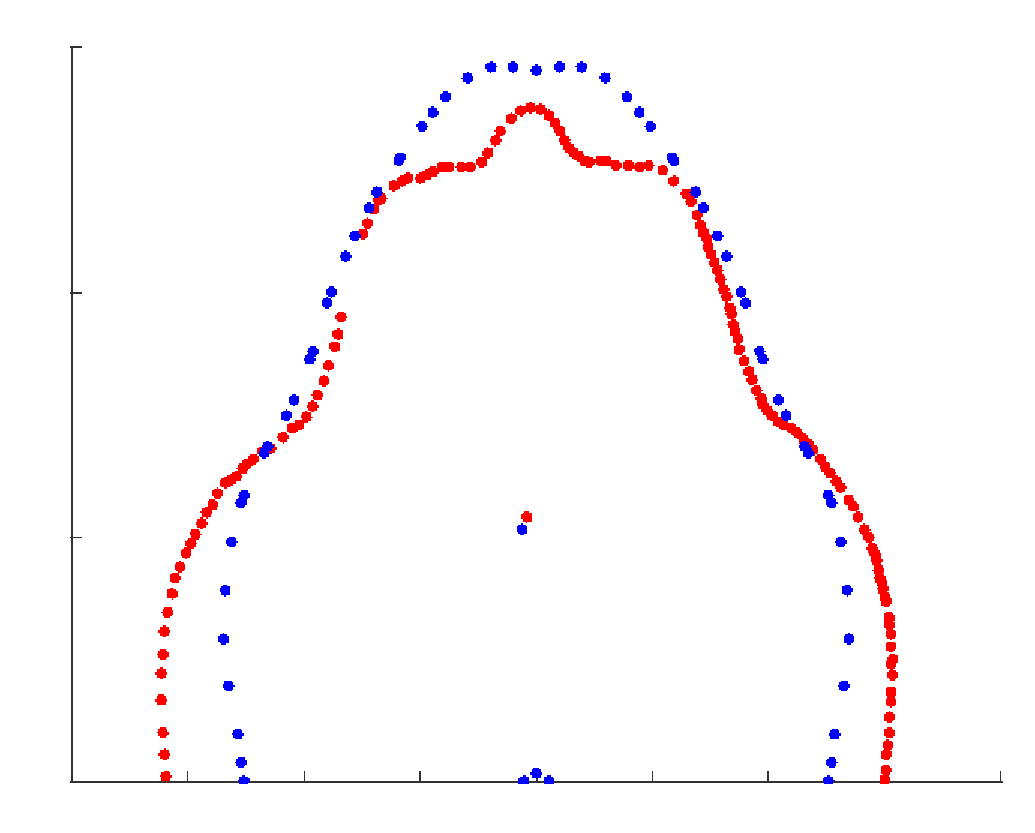
\includegraphics[width=0.3\textwidth]{hung-9.eps}
      }
       \subfloat[t = 0.0382 ]{%
      \includegraphics[width=0.3\textwidth]{hung-10.eps}
      }
 \caption{Interface and center of mass Gerris simulation data(BLUE) with \cite{Hung2011} experimental data(RED), Contact Angle $150^o$}
 \label{Fig:gs5}
 \end{figure}
 
 \begin{figure}[H]
 \includegraphics{y_com_hung.eps}
 \caption{y coordinate of center of mass of droplet to time}
 \label{Fig:y_com}
\end{figure}

The interface points and center of mass from the experimental data(\cite{Hung2011}) were extracted and compared with Gerris simulation data. 
The simulation results were in agreement with experiment before the impact. Just after the impact (See Figure \ref{Fig:gs5} (a),(b)) the contact line and the contact angle is coinciding with 
the experimental but as the contact line started to move in the (c) \& (d), the simulation interface did not moved because of the no slip boundary condition and also has the contact 
contact angle. From (c) to (j) the results are very different from what is observed in the experiment. The vertical position of center of mass is less sensitive to the impact surface.
Figure \ref{Fig:y_com} shows the variation of vertical height of center of mass of droplet with respect to time. It looks like a damped oscillation.  

\begin{figure}[H]
 \centering
 \subfloat[t = 26.2 ]{%
      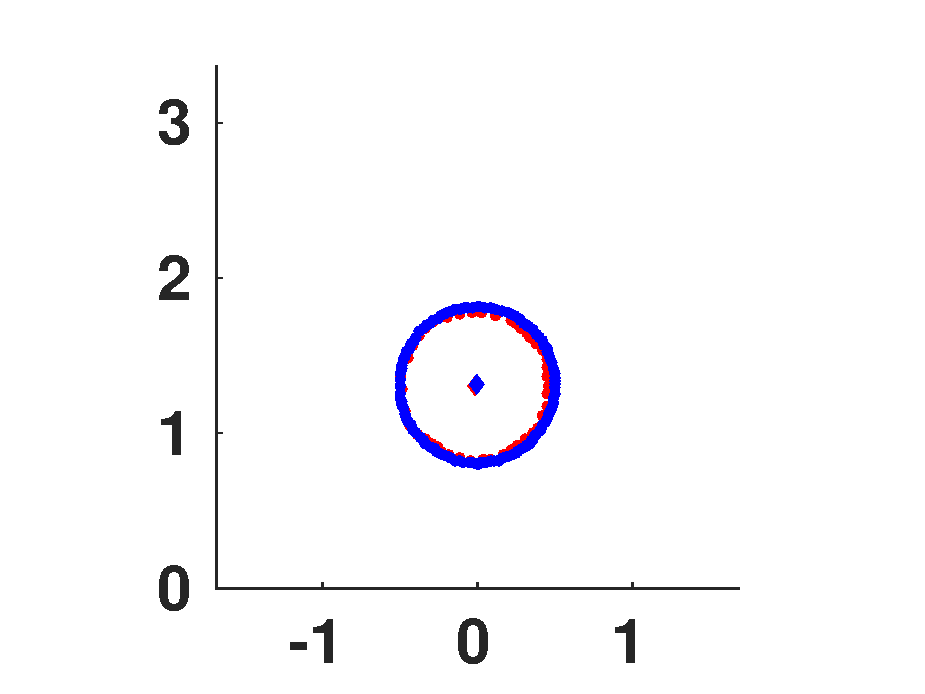
\includegraphics[width=0.3\textwidth]{clanet-1.eps}
      }
  \subfloat[t = 27.1 ]{%
      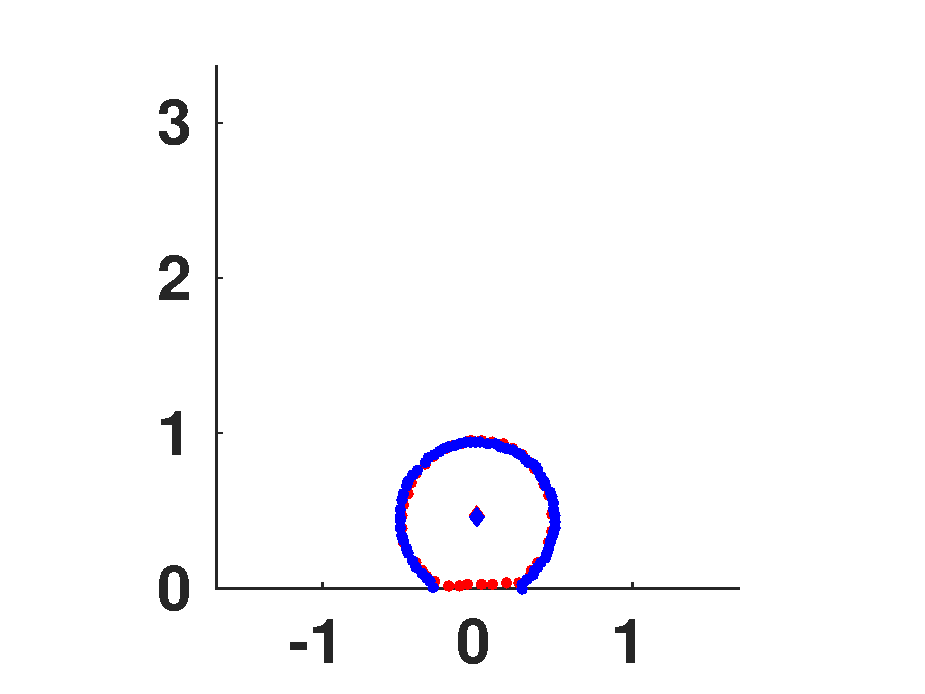
\includegraphics[width=0.3\textwidth]{clanet-2.eps}
      } 
       \subfloat[t = 28.0 ]{%
      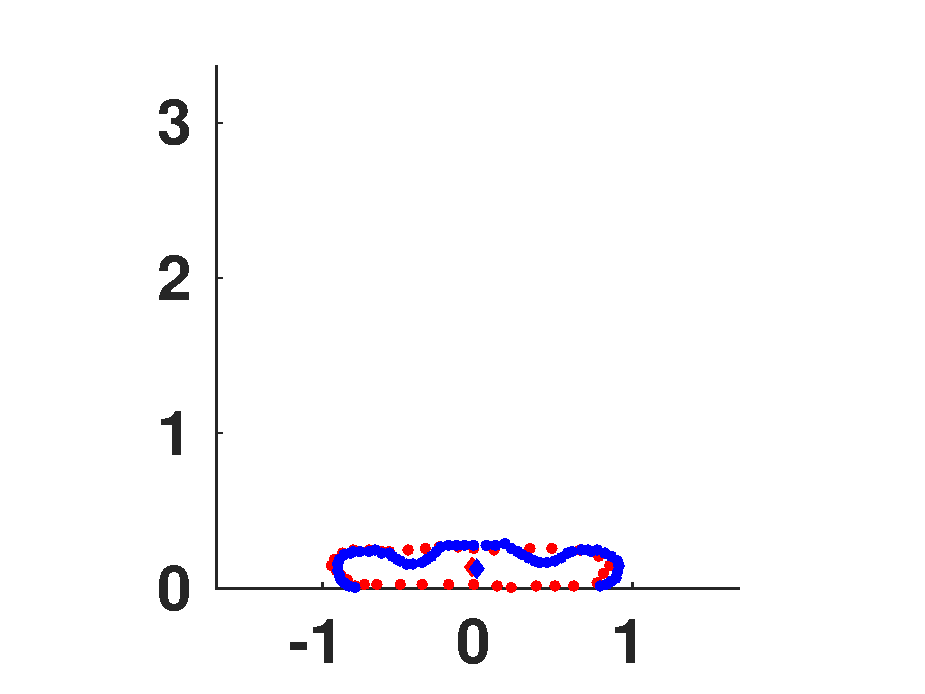
\includegraphics[width=0.3\textwidth]{clanet-3.eps}
      }\\
       \subfloat[t = 28.9 ]{%
      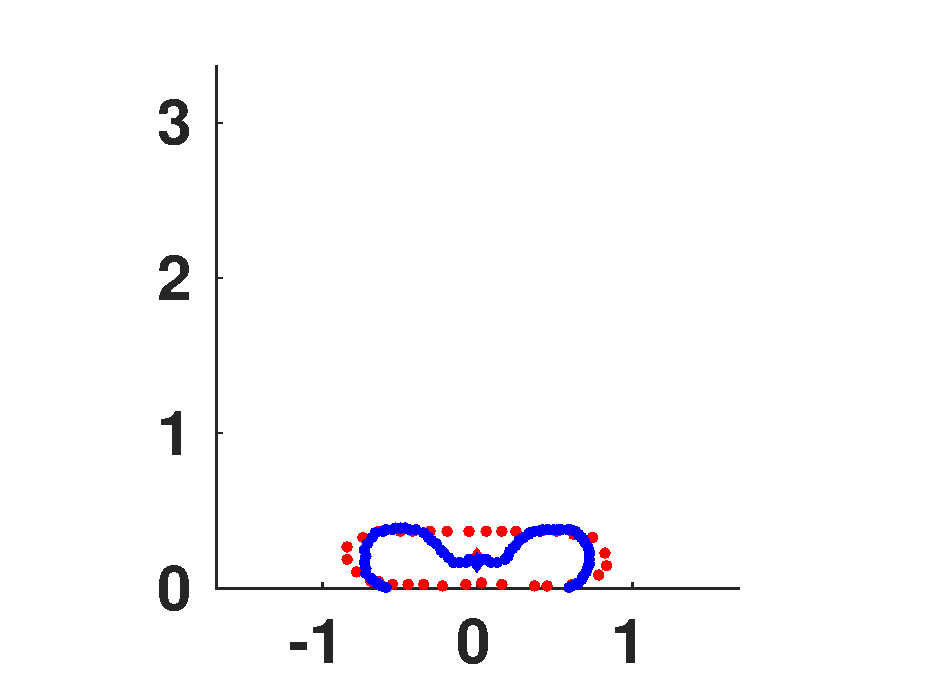
\includegraphics[width=0.3\textwidth]{clanet-4.eps}
      }
    \subfloat[t = 29.8 ]{%
      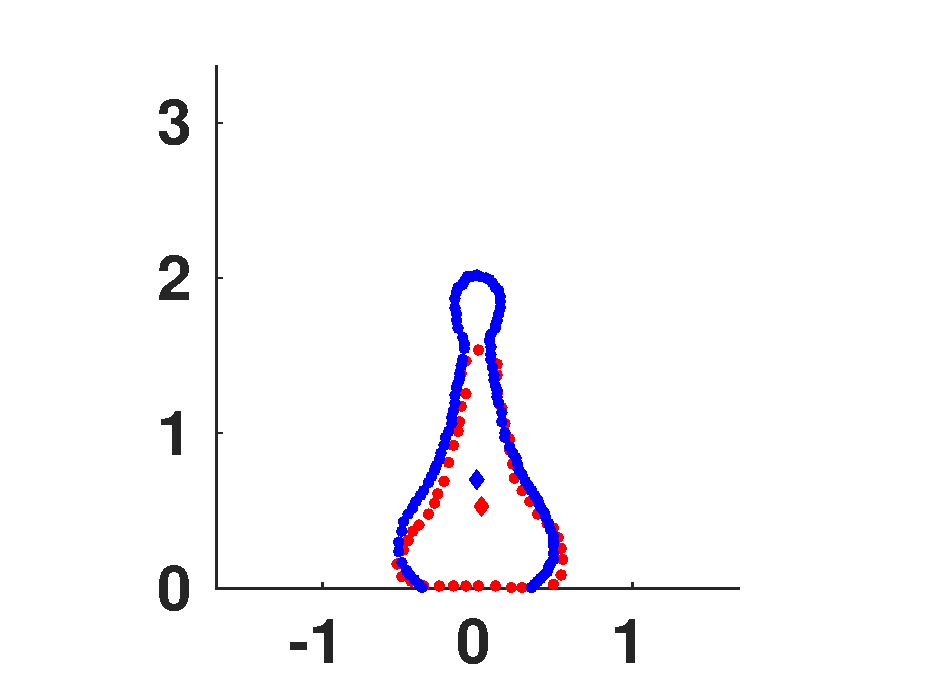
\includegraphics[width=0.3\textwidth]{clanet-5.eps}
      }
       \subfloat[t = 30.7 ]{%
      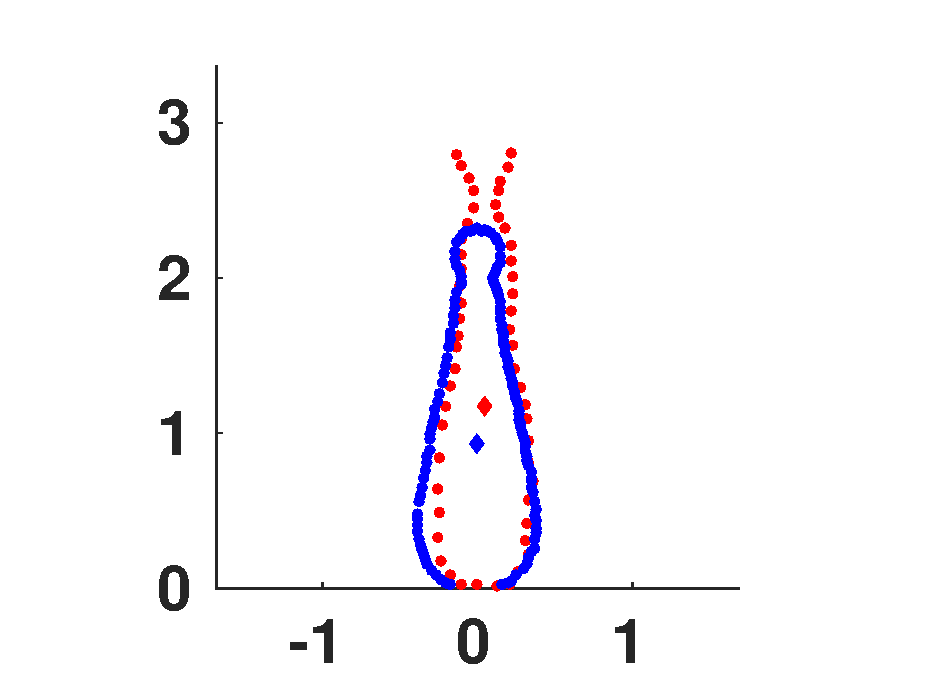
\includegraphics[width=0.3\textwidth]{clanet-6.eps}
      }\\
       \subfloat[t = 31.6 ]{%
      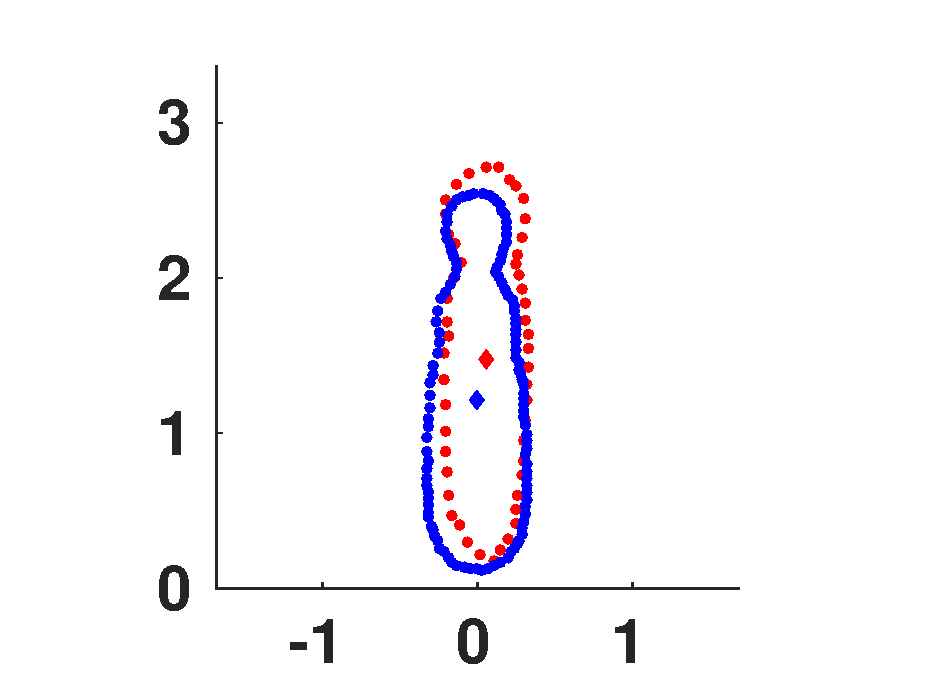
\includegraphics[width=0.3\textwidth]{clanet-7.eps}
      }
       \subfloat[t = 32.5 ]{%
      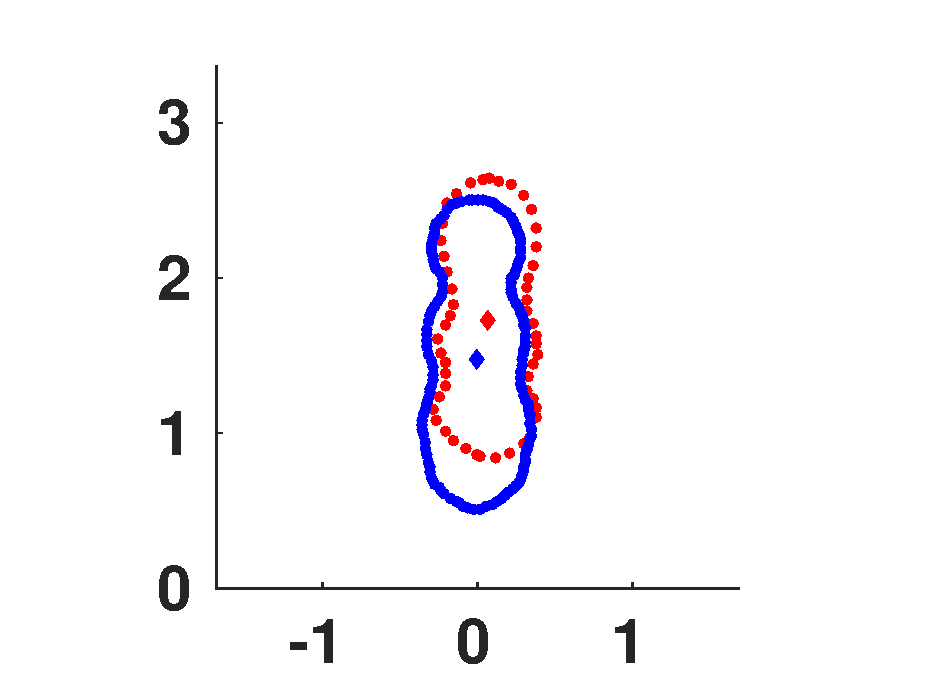
\includegraphics[width=0.3\textwidth]{clanet-8.eps}
      }
       \subfloat[t = 33.4 ]{%
      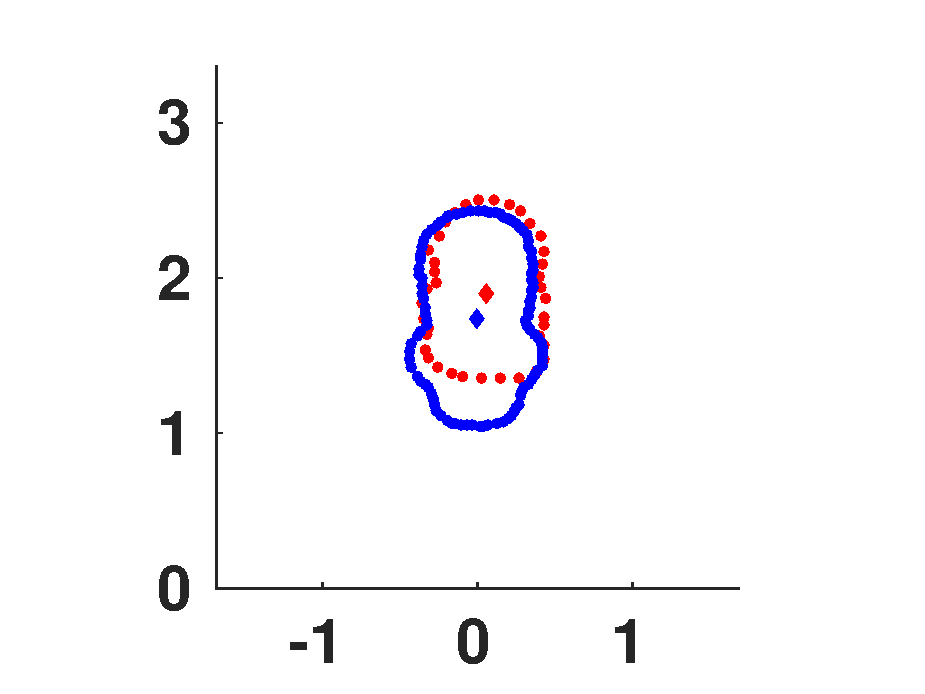
\includegraphics[width=0.3\textwidth]{clanet-9.eps}
      }
 \caption{Interface Gerris simulation data(BLUE) with \cite{Clanet2004} experimental data(RED) Contact Angle $170^o$}
 \label{Fig:gs6}
 \end{figure}
 \cite{Clanet2004}  also shown that droplet impacting on superhydrophobic behaves like a balloon filled with fluid in some region of parameters,
 where the movement of contact line is restricted and the boundary condition for velocity can be taken as no-slip. 
 \cite{Clanet2004} study involved superhydrophobic surfaces and with contact angle of  $170^o$. We made a comparison with Gerris simulation with static contact angle
 boundary condition and no slip  at surface (See Figure \ref{Fig:gs6}). It can be seen that superhydrophobic surfaces has minimum spreading and has minimal effect on 
 the dynamics of droplet impact.
 
 \begin{figure}[H]
 \centering
 \subfloat[t = 15.6 ]{%
      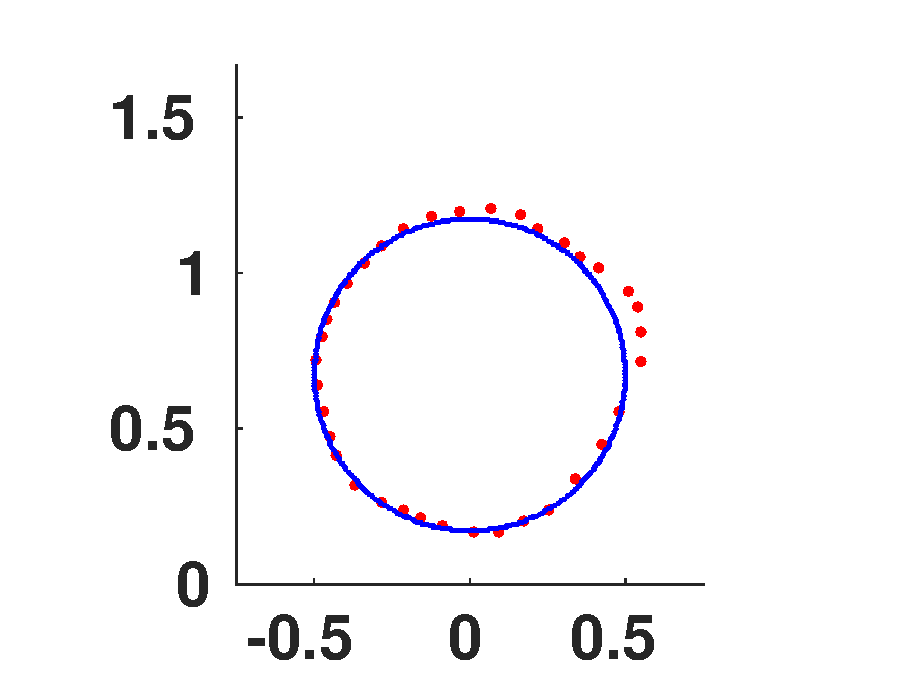
\includegraphics[width=0.3\textwidth]{wang-1.eps}
      }
  \subfloat[t = 16.0 ]{%
      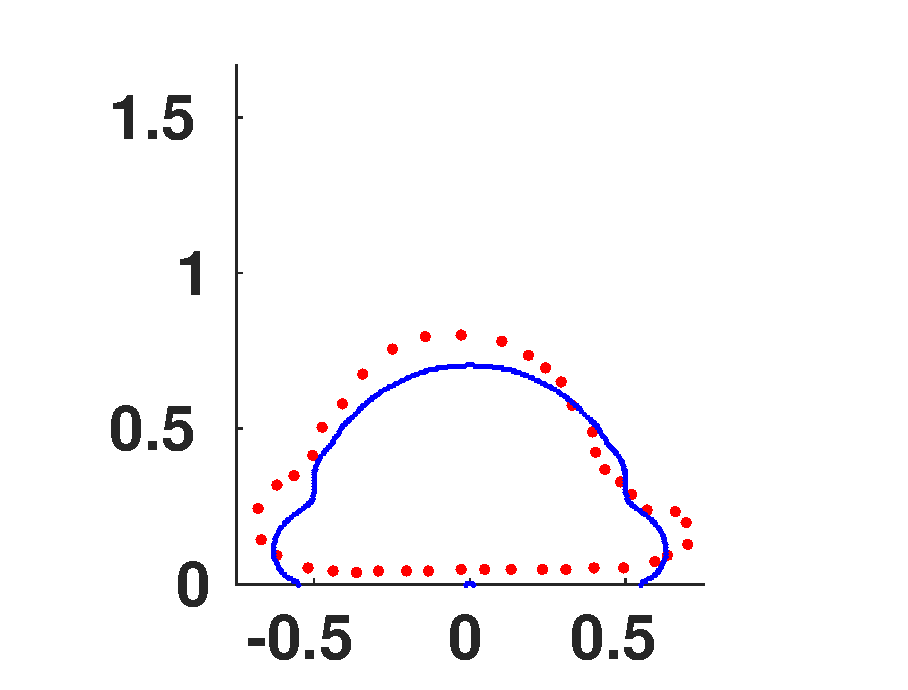
\includegraphics[width=0.3\textwidth]{wang-2.eps}
      } 
       \subfloat[t = 17.0 ]{%
      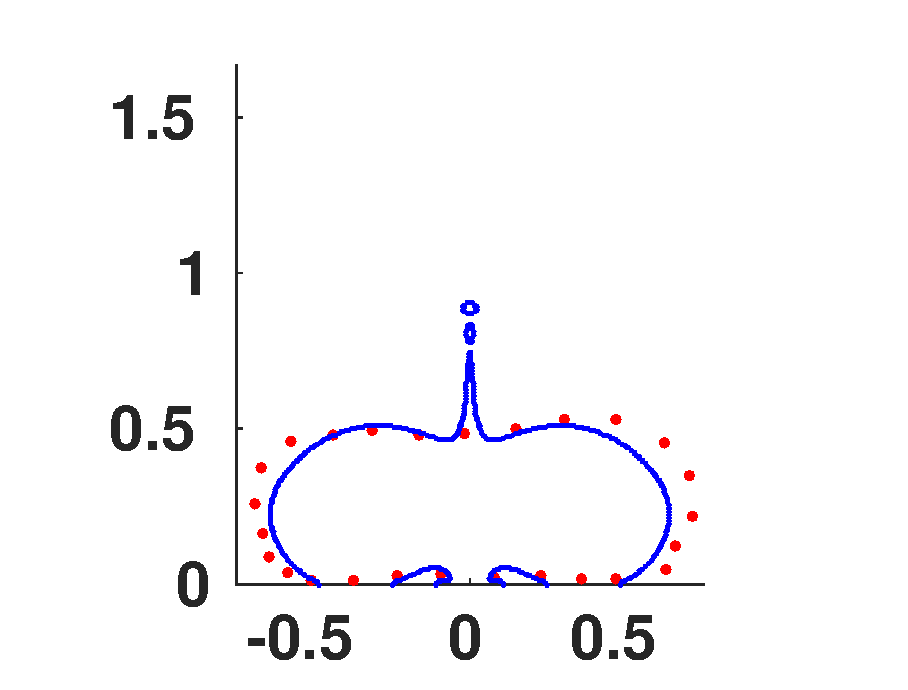
\includegraphics[width=0.3\textwidth]{wang-3.eps}
      }\\
       \subfloat[t = 18.1 ]{%
      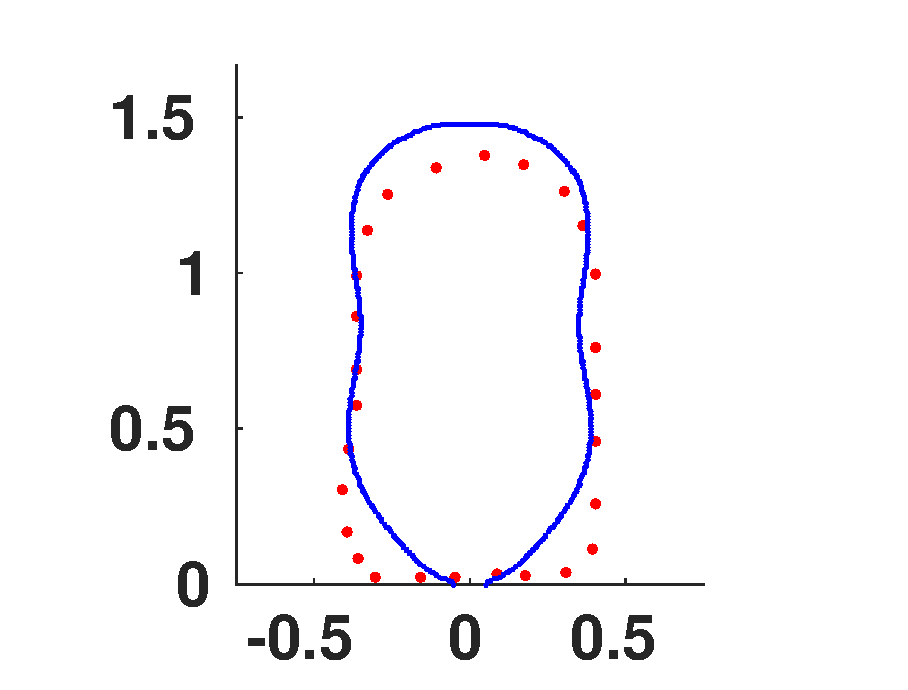
\includegraphics[width=0.3\textwidth]{wang-4.eps}
      }
    \subfloat[t = 19.0 ]{%
      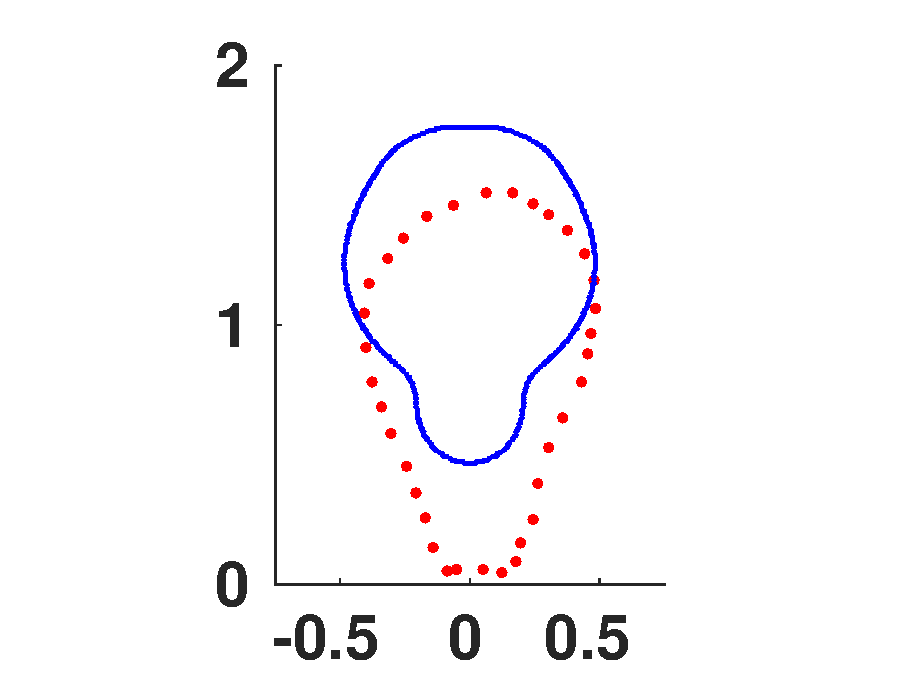
\includegraphics[width=0.3\textwidth]{wang-5.eps}
      }
       \subfloat[t = 19.5 ]{%
      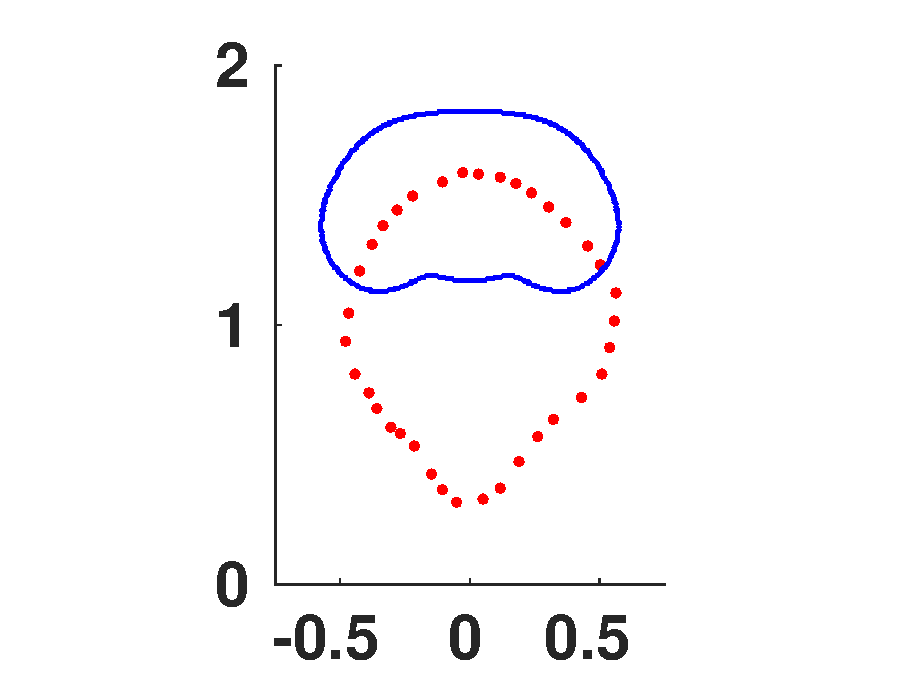
\includegraphics[width=0.3\textwidth]{wang-6.eps}
      }
    \caption{Interface Gerris simulation data(BLUE) with \cite{Wang2007} experimental data(RED) Contact Angle $163^o$ }
 \label{Fig:gs7}
 \end{figure}   
  \begin{figure}[H]
 \centering
 \subfloat[t = 15.6 ]{%
      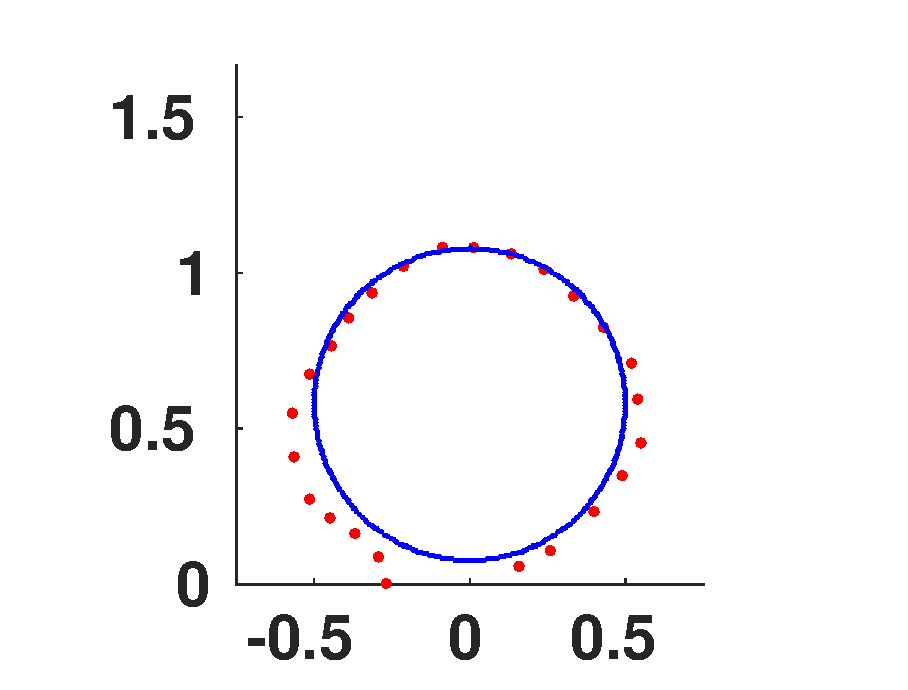
\includegraphics[width=0.3\textwidth]{wang-140-1.eps}
      }
  \subfloat[t = 16.6 ]{%
      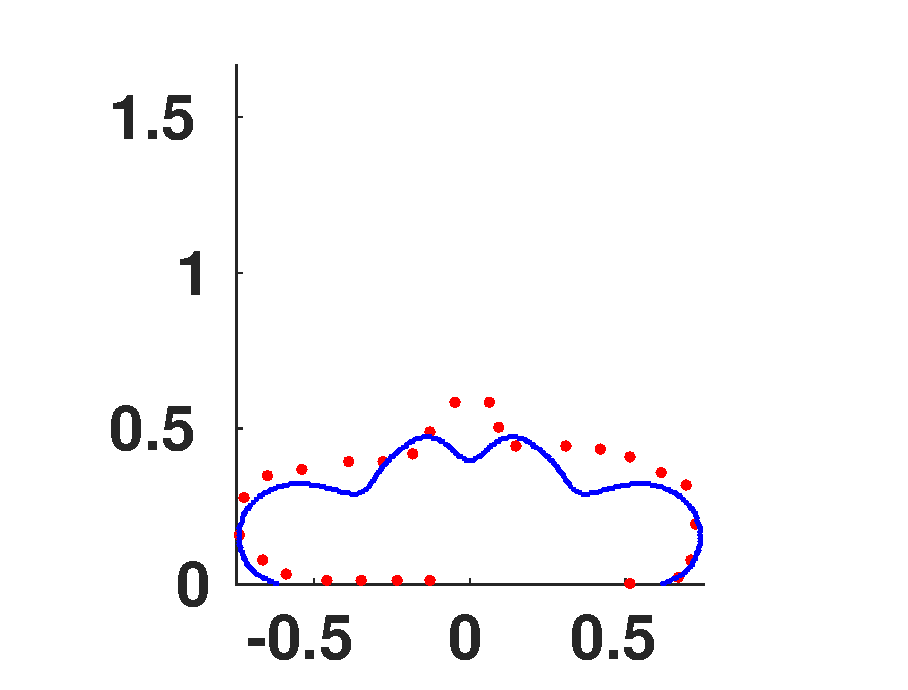
\includegraphics[width=0.3\textwidth]{wang-140-2.eps}
      } 
       \subfloat[t = 17.5 ]{%
      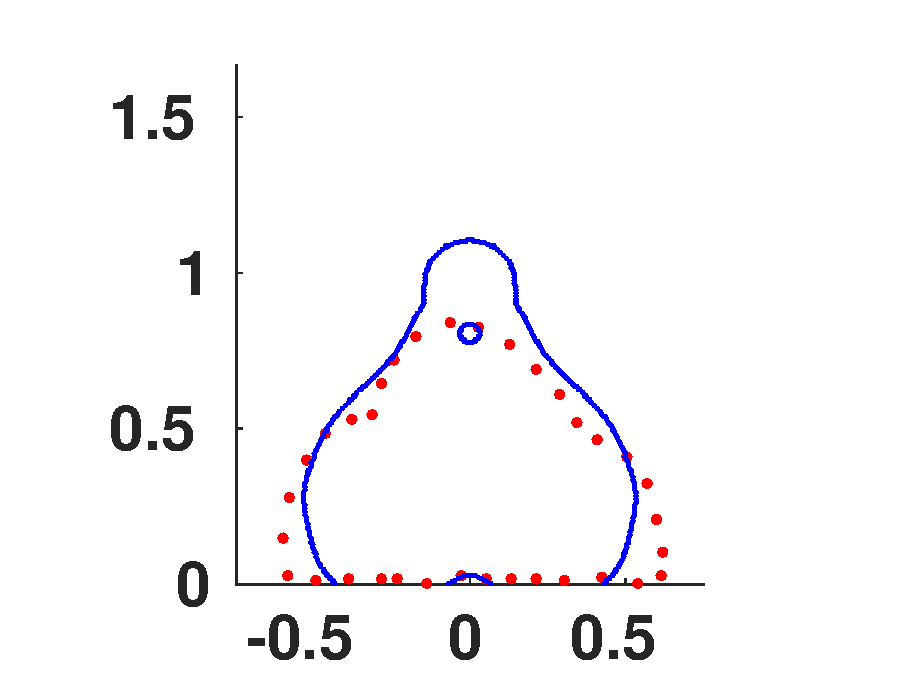
\includegraphics[width=0.3\textwidth]{wang-140-3.eps}
      }\\
       \subfloat[t = 20.4 ]{%
      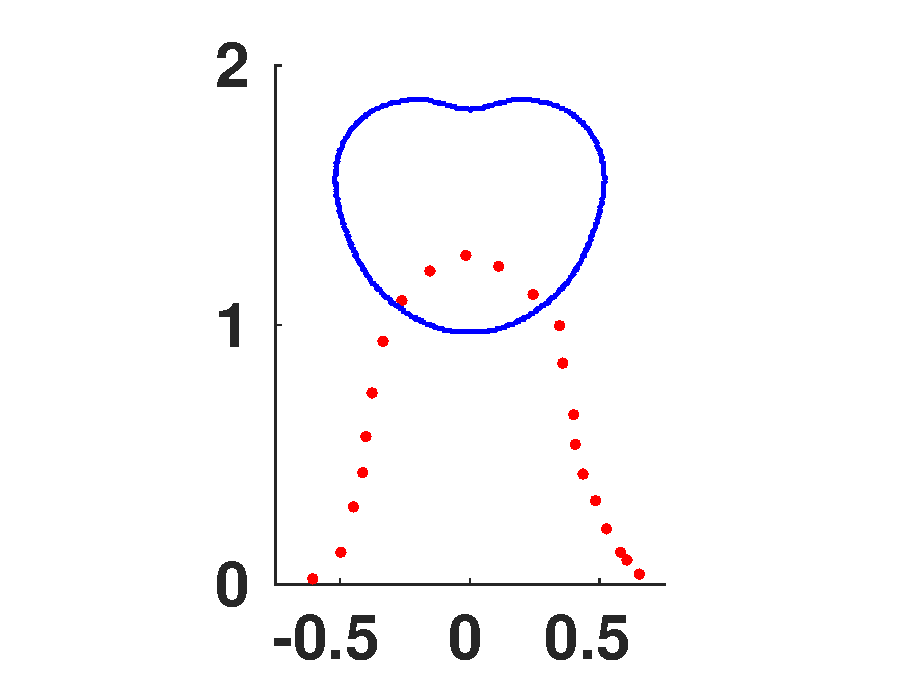
\includegraphics[width=0.3\textwidth]{wang-140-4.eps}
      }
    \subfloat[t = 21.9 ]{%
      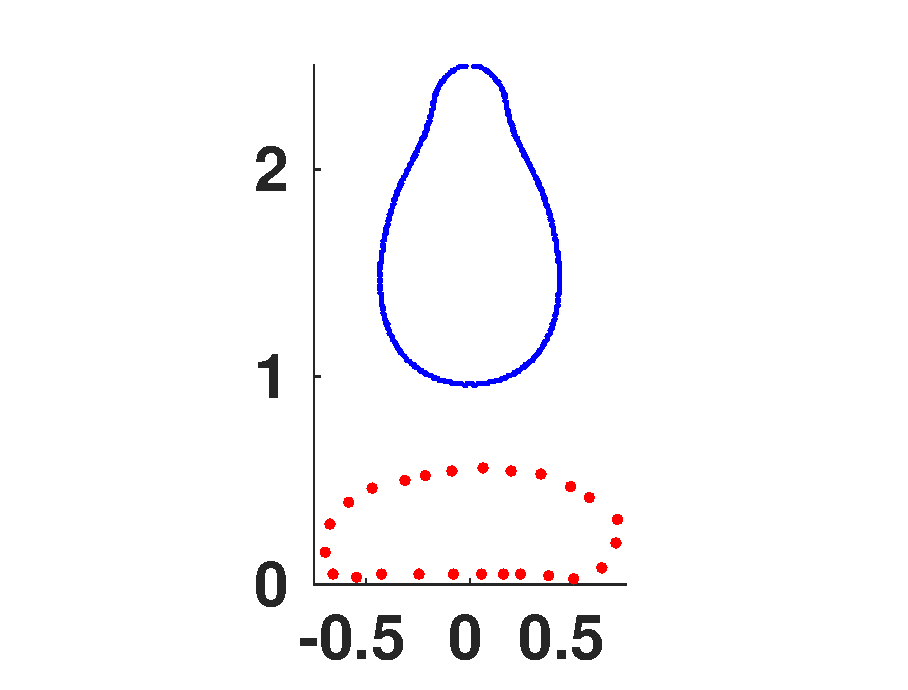
\includegraphics[width=0.3\textwidth]{wang-140-5.eps}
      }
       \subfloat[t = 24.6 ]{%
      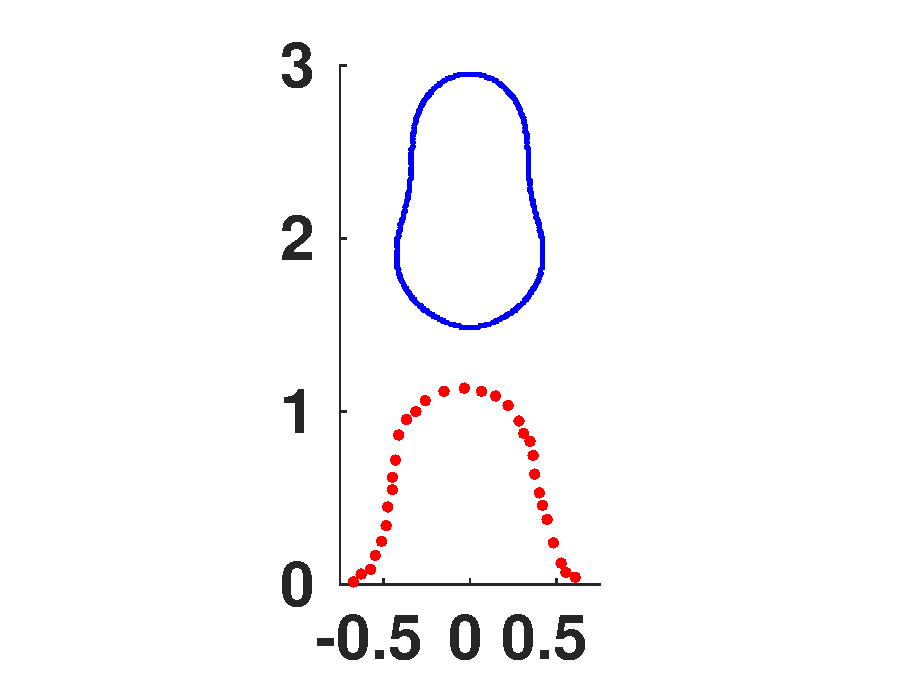
\includegraphics[width=0.3\textwidth]{wang-140-6.eps}
      }
    \caption{Interface Gerris simulation data(BLUE) with \cite{Wang2007} experimental data(RED) Contact Angle $140^o$}
 \label{Fig:gs8}
 \end{figure}   
A comparison with \cite{Wang2007} (See Figure \ref{Fig:gs7}), the surface has a contact angle of $163^o$, also corroborate the fact that the static contact angle conditions
are a good approximation for the solution of droplet impact on superhydrophobic surfaces.\\
 From above comparisons on superhydrophobic surfaces, we can approximate that the static contact line boundary conditions have negligible effect on droplet impact and we can have
 valid approximations for the dynamics involved.  In the light of above comparisons we want to study some of the problems in superhydrophobic surfaces 
 as below:-  
\begin{enumerate}
\item Motion of center of mass of droplet 
 \item Droplet impact on inclined plane
 \item Droplet impact inclined to the plane
 \item Oscillations of droplet after impact
 \item Droplet breakup after impact
\end{enumerate}

\section{Conclusion}
Due to this limitation of Gerris code, future work involves development of a multiphase Navier-Stokes solver and to implement the moving contact line and dynamic contact line 
model in it. Till then we will use Gerris code to observed some simpler outcomes of droplet impact on superhydrophobic surfaces.
Our code will mimic the actual droplet impact after implementation of the contact models. We will
look to explain some aspects of this phenomena through a simpler mathematical model.


% \begin{figure}
%  \centering
%  \subfloat[ ]{%
%       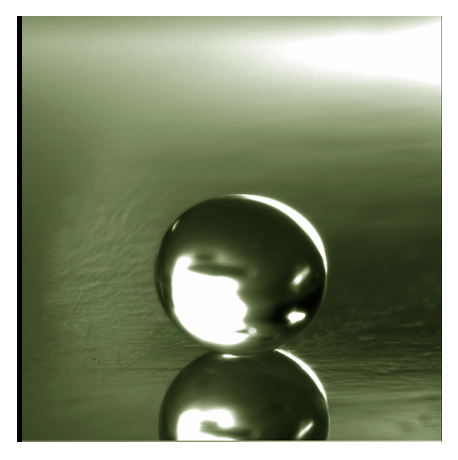
\includegraphics[width=0.3\textwidth]{droplet_c1.eps}
%       }
%   \subfloat[t = 27.1 ]{%
%       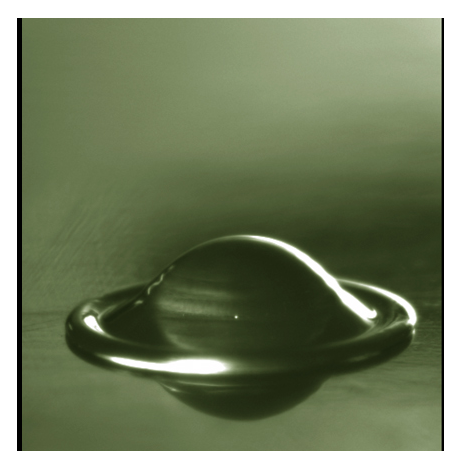
\includegraphics[width=0.3\textwidth]{droplet_c2.eps}
%       } 
%        \subfloat[t = 28.0 ]{%
%       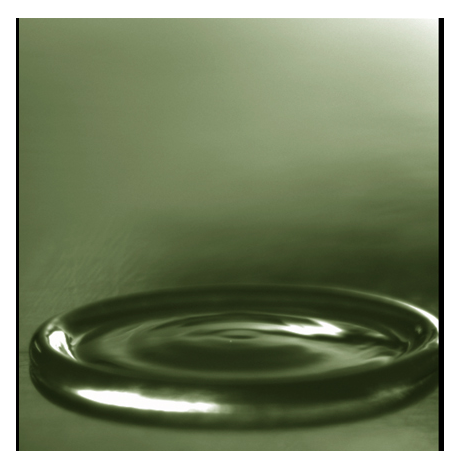
\includegraphics[width=0.3\textwidth]{droplet_c3.eps}
%       }
%   \caption{Moving contact line during impact}
%   \label{Fig:contact_line}
%   \end{figure}
